
\section{Overview}

For some time, there has been a need for a \cpp\ class embodying the
information contained in the Review of Particle Properties\cite{pdg}.
We have written HepPDT to fill this need.  
HepPDT allows access
to particle name, particle ID, charge, nominal mass,  total width,
spin information, color information, and constituent particles.
HepPDT is designed to be used by any Monte Carlo generated particle class. 
Generated particles could, if desired, contain a
pointer to the particle data information found in the HepPDT
particle data table.  

\subsection{HepPDT Design}

HepPDT has been designed to be used by any Monte Carlo particle generator
or decay package.  It contains only generic particle attributes.
In principle, all information which can be found in
the Review of Particle Properties\cite{pdg} can be encapsulated in HepPDT.
However, because the user base has not found the inclusion of decay table 
information useful, HepPDT 3.xx no longer contains any decay information.

HepPDT stores particle information such as charge and nominal mass  
in a table which is accessed by a particle ID number.  
The particle ID number is defined according to the Particle Data Group's
Monte Carlo numbering scheme\cite{scheme}.  

Methods are provided to create ParticleDataTable objects from
Pythia, Herwig, Isajet, QQ, and EvtGen.  Methods
are also provided to facilitate creation of custom particle 
information.  A ParticleDataTable object may be created from
multiple information sources.

The design requires that ParticleDataTable objects must be fully created
before they are used.  Multiple data tables are allowed.  Although
potentially dangerous, we recognize that this is also a powerful option.

Figure~\ref{fig:a} shows the interactions of the basic classes.

\begin{figure}
  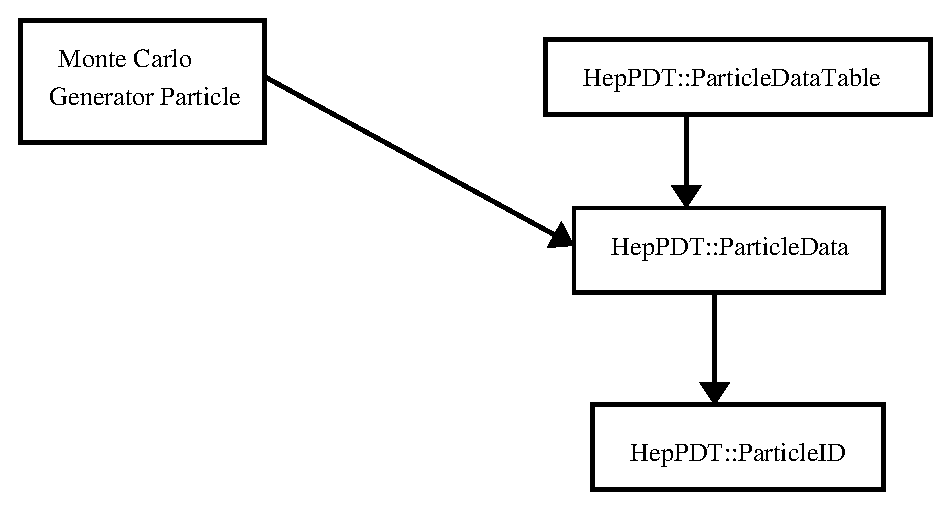
\epsfig {file=HepPDT-class.eps, width=18cm }
\caption{HepPDT Classes: 
Particle information is accessed either by a pointer to ParticleData from any
Monte Carlo generated particle or by lookup with a string or ID.  
ParticleData contains particle information such as mass, charge,
and total width.  
The ParticleDataTable contains a map of ParticleData objects,
referenced by ParticleID.
ParticleData has methods to access all relevant information. }
\label{fig:a}
\end{figure}

\subsection{HepPDT Classes}

The ParticleDataTable class contains a map of ParticleData
which is keyed on the ParticleID class.  

The ParticleID
class can be used to retrieve all the information that is implied 
in the particle ID (\eg, charge and quark content).   Boolean methods
(such as isMeson, isBaryon, hasBottom, and hasTop) are provided
for ease of searching for various types of particles.

The ParticleData class includes particle name, particle ID, charge,
mass, total width with cutoffs, spin information, color information, 
and constituent particles (\eg, quark content).  


\section { Particle Numbering Scheme }

The Particle Data Group \cite{pdg} provides a standard particle 
numbering scheme.
This nubmering scheme is decscribed in full detail in
reference \cite{scheme}.

HepPDT uses the translation methods in HepPID.\cite{heppid}

\subsection { ParticleID }

The HepPDT::ParticleID class  
provides methods to return all the information
which can be extracted or inferred from the particle ID (PID).
It is expected that any 7 digit number used as a PID will adhere to the 
rules of the Monte Carlo Particle Numbering Scheme published by the
PDG.\cite{pdg}

The ParticleID class considers any particle with 
an ID less than 100 a "fundamental" particle.

In most cases, a user can define particles not already in the
Particle Data Table without needing to extend the numbering scheme.
A previously unknown particle can be assigned a valid PID by
following the rules in the "Review of Particle Physics".\cite{pdg}

If the user wishes to force the decay chain 
$D^* \rightarrow D^0 \pi^0, D^0 \rightarrow K^- \pi^+ \pi^0 \pi^0$,
a user might define a special $D^0$ which only decays to 
$K^- \pi^+ \pi^0 \pi^0$, leaving any $D^0$ produced elsewhere to decay normally.
The PID for a normal $D^0$ is 421.  The PID for the special $D^0$
might be 6000421.   This new PID might be used in several different jobs
for $D^0$ particles with different forced decay modes.
(EvtGen defines these special particles as aliases in the decay table.
The TableBuilder class handles the aliases appropriately without needing
to create a new PID for the particle alias.)

\begin{center}
\begin{tabular}{ll}
 & ParticleID( int pid = 0 ); \\
 & ParticleID( const ParticleID \& orig );  \\
 & ParticleID \& operator=( const ParticleID \& );  \\
void & swap( ParticleID \& other );  \\
bool  & operator $<$  ( ParticleID const \& other ) const;  \\
bool   &operator == ( ParticleID const \& other ) const;  \\
 \\
int   &  pid( )        const;  \\
int & abspid( )        const;  \\
 \\
bool & isValid( )   const; \\
bool & isMeson( )   const;\\
bool  & isBaryon( )  const;\\
bool  & isDiQuark( ) const;\\
bool & isHadron( )  const; \\
bool & isLepton( )  const; \\
bool & isNucleus( )  const; \\
 \\
bool & hasUp( )      const; \\
bool & hasDown( )    const;\\
bool & hasStrange( ) const;\\
bool & hasCharm( )   const;\\
bool & hasBottom( )  const;\\
bool & hasTop( )     const;\\
 \\
int  & jSpin( )        const; \\
int  & sSpin( )        const;\\
int  & lSpin( )        const; \\
int & fundamentalID( ) const; \\
Quarks & quarks( ) const; \\
int & threeCharge( ) const; \\
int & A( ) const;\\
int & Z( ) const;\\
unsigned short & digit(location) const; \\
\end{tabular}
\end{center}

\section { Particle Properties }

Particle data information is stored in HepPDT::ParticleDataTable, 
which is a map of HepPDT::ParticleData objects
that are referenced by HepPDT::ParticleID. 
The design envisions that generated particles will contain links
to the relevant  HepPDT::ParticleData object.

\subsection { Reading Particle Data information }

HepPDT can accept particle data information from a variety of sources.
To fill HepPDT::ParticleDataTable, 
the user creates an empty ParticleDataTable object
and then calls HepPDT::TableBuilder methods to read the information 
from an input stream.
Information may be read from as many input streams as desired.
In case of conflicts, previous information will be overwritten.
All information is kept in temporary objects until the TableBuilder destructor
is called.  
The TableBuilder destructor then creates the ParticleData objects owned
by ParticleDataTable.  

The following code fragment reads Pythia input from a flat file.
Examples reading input from other sources are in Appendix \ref{readdata} 
and also in the example subdirectory. 

\begin{verbatim}
#include <fstream>

#include "HepPDT/TableBuilder.hh"
#include "HepPDT/ParticleDataTable.hh"
#include "HepPDT/TempParticleData.hh"

    const char infile[] = "data/pythia.tbl";
    // open input file
    std::ifstream pdfile( infile );
    if( !pdfile ) { 
      std::cerr << "cannot open " << infile << std::endl;
      exit(-1);
    }
    // construct empty PDT
    HepPDT::ParticleDataTable datacol( "Pythia Table" );
    {
        // Construct table builder
        HepPDT::TableBuilder  tb(datacol);
	// read the input - put as many here as you want
        if( !addPythiaParticles( pdfile, tb ) ) 
	      { std::cout << "error reading pythia file " << std::endl; }
    }	// the tb destructor fills datacol
\end{verbatim}

The Particle Data Group provides a table of particle masses and widths for known
particles.  This table,  pdg\_mass.tbl, is distributed with the HepPDT package.
This information is also available from specific generators, often as
flat files.  

By request, a simple table, particle.tbl, of particle masses and widths has 
been added to HepPDT.  This table is intended to be a complete list of useful
particles.   Use the addParticleTable() free function, defined in 
TableBuilder.hh, to parse this file.

\subsection { Accessing Particle Data information }

The following code fragment accesses pion and muon information.
Refer to the Appendices for a listing of particle ID numbers.
\begin{verbatim}
    std::ofstream wpdfile( outfile );
    HepPDT::ParticleDataTable db( "my Table" );
    ......
    HepPDT::ParticleData * pd = datacol.particle( HepPDT::ParticleID(111) );
    pd->write(wpdfile);
    double mumass = datacol.particle( HepPDT::ParticleID(13) )->mass();
\end{verbatim}

In principle, all information in the PDG may be obtained from ParticleData
access methods.

\begin{center}
\begin{tabular}{ll}
  std::string const \&         & name()        const;  \\    
  ParticleID                  & ID()          const; \\
  int                         & pid( )        const; \\
  double                      & charge()      const; \\
  double                      & color()       const; \\
  SpinState                   & spin()        const; \\
  Measurement                 & mass()        const; \\
  Measurement                 & totalWidth()  const; \\
  Measurement                 & lifetime()    const; \\
  int                         & numConstituents() const; \\
   Constituent          & constituent( unsigned int i ) const; \\
   ParticleID           & constituentParticle( unsigned int i ) const; \\
  ResonanceStructure const *  & resonance()   const; \\
 \\
  bool & isMeson( )   const; \\
  bool & isBaryon( )  const; \\
  bool & isDiQuark( ) const; \\
  bool & isHadron( )  const; \\
  bool & isLepton( )  const; \\
  bool & isNucleus( ) const; \\
  bool & hasUp()      const; \\
  bool & hasDown()    const; \\
  bool & hasStrange() const; \\
  bool & hasCharm()   const; \\
  bool & hasBottom()  const; \\
  bool & hasTop()     const; \\
   \\
   void & write( std::ostream \& os ) const; \\
\end{tabular}
\end{center}

\subsection{ The Measurement Class }

Some tables contain errors on mass and width values.
To keep this error information available, we wrote a simple HepPDT::Measurement
class which contains a double value and a double error on the value.
If you reference it with a double, Measurement returns the value.

\begin{center}
\begin{tabular}{ll}
 & Measurement( double value, double sigma ); \\
 & Measurement( const Measurement \& orig );  \\
 & Measurement \& operator=( const Measurement \& );  \\
void & swap( Measurement \& other );  \\
bool  & operator $<$  ( Measurement const \& other ) const;  \\
bool   & operator == ( Measurement const \& other ) const;  \\
   double  &  value()  const;\\
   double   & sigma()  const;\\
   operator & double() const;\\
\end{tabular}
\end{center}

\subsection{ Particles Not in the Table }

If a particle definition has not been added to the ParticleDataTable,
a lookup of that particle with either operator[] or the particle() method
will return a null pointer to ParticleData.   However, there are some instances
where you might want to create a ParticleData dynamically.  Specifically,
this is handy when dealing with the heavy ions produced dynamically by
Geant4.

A abstract plugin class, ProcessUnknownID, is now available that allows you
to specify what happens when you try to lookup a particle ID that is not
in the table.  The plugin class contains processUnknownID() which returns
a pointer to a ParticleData object.  
This pointer should be null if no ParticleData object is defined.
The unknown ParticleID and a const reference to ParticleDataTable are 
passed to processUnknownID().
To use this class, create your own MyProcessUnknownID class
which inherits from ProcessUnknownID.  
You only need to define a constructor and 
MyProcessUnknownID::processUnknownID( ParticleID,  const ParticleDataTable \& ).

By default, ParticleDataTable behaves exactly as before, 
returning a null pointer to ParticleData.  HepPDT also contains the
HeavyIonUnknownID class which will create a ParticleData for an unknown
nuclear fragment.  Code fragments are shown in appendix \ref{unknownID}.

\section{Conclusions}

HepPDT provides access to all useful particle data properties
and is designed to be used with any generated particle.    
The HepPDT home page is http://cepa.fnal.gov/psm/heppdt/.
